\subsection{Dataset}
A dataset of ten novels and a play was collected from the internet, with at
least three summaries each. The books are mainly fictional classics, due to
their popularity on summary resources and often the expiration of their
copyright. Most of the summaries are sourced from CliffsNotes, SparkNotes and
GradeSaver. The books and summaries both vary quite vastly in length. All the
documents were saved as or converted to text files, to facilitate consistency
and ease of manipulation in Python.

\subsection{Evaluation}
Aside from simply reading the summarization outputs of the algorithm, two
quantitative measures are used to evaluate them.
The nltk.translate.bleu\_score toolkit has a function, corpus\_blue, which can
be used for BLEU evaluation. BLEU was originally used for translations, but is
now also used to evaluate summaries and is based on precision scores of
n-gram overlaps between documents and references. The corpus\_blue allows for
varying weights of 1- to 4-grams, and for multiple golden references. 

In table~\ref{table:bleu_huckfinn}, example scores of running this BLEU
evaluation can be seen. In each case, one online summary was evaluated against
the other three as golden references. For pure 1-grams, the scores are always
higher than 2-grams, and indeed they were almost zero for 3- and 4-grams.
Another remark is that while scores over 0.6 seem quite high, the CliffsNotes
score is a low outlier at only 0.295 for the 1-gram case. Finally, it must be
noted that increasing the number of references also increases the score.
Because there are more versions of what a ``correct'' summary is, there is
probably also more overlap of the remaining summary to them. Because it is not
easy to obtain more summaries, the availability of only three to four per book
must simply be kept in mind as a limitation when it comes to evaluation.

\begin{table}[H]
	\centering
	\caption{Example BLEU 1-gram and 2-gram evaluation for online summaries of the Adventures of Huckleberry Finn.}\label{table:bleu_huckfinn}
	\begin{tabular}{l l l }
		\toprule
		\textbf{}   & \textbf{1-gram} & \textbf{2-gram} \\ \midrule
		CliffsNotes & 0.295           & 0.127           \\ \midrule
		SparkNotes  & 0.646           & 0.260           \\ \midrule
		GradeSaver  & 0.655           & 0.262           \\ \midrule
		Wiki   & 0.646           & 0.234           \\
		\bottomrule
	\end{tabular}
\end{table}

Additionally, ROUGE (recall-oriented understudy for gisting evaluation) is also
used for evaluation; the score is based on recall of n-gram overlaps between
system and golden summaries. Because higher n-gram scores are so low, 1- and 2-
grams of each BLEU and ROUGE were the main metrics used. In evaluating, words
were stemmed, stop-words were accounted for and punctuation was removed, in
order to focus on content rather than phrasing.

\subsection{Results}
Because of the novelty of the method, there were no established baselines to
compare to. As ROUGE and BLEU scores would also vary wildly with the dataset
used, it would also not make sense to compare these to other studies. In terms
of purely quantitative scores, promising results were obtained, in the sense
that the system summaries scored similarly to the golden summaries against each
other.

In the experiments, the effect of changing various parameters was examined. The
first of these was the sizes of the sections that the book was broken into.
This was varied between 10 and 100 sentences, while the number of sentences out
from each chunk was kept constant at 5 sentences. In
Appendix~\ref{appendix:countfigs}, figure~\ref{fig:bleus_okay} shows an example of these
results for the Alchemist. From this, it was found that performance was roughly
constant for sentence chunks up to 50, after that it drops. This indicates that
when output sentences drop to less than 10\% of input sentences in each step,
the information retention drops.

In another experiment, the chunk size was kept constant at 50 sentences, but
the number of sentences output from these was varied between 1 and 45. From
figure~\ref{fig:bleus}, it can be seen that there is an optimum at 10 sentences
out for 50 sentences in, for the Alchemist but also observed in other books.
More interestingly, these experiments were repeated both with and without using
the important words to weight sentences. While weighting did not make any
significant difference in the BLEU-1 score, it consistently improved BLEU-2
score. This indicates that more important and informative sentences were
selected due to the weighting. Additionally, BLEU-1 scores around 0.5 and
BLEU-2 around 0.15, which are each only around 0.6 lower than golden references
evaluated against the others.

We also ran the ROUGE evaluation script, which involve evaluating a given
summary against all the other available summaries for that book. The ROUGE
results for the Alchemist are seen in table~\ref{tab:rouge-alchemist}. For
generating our summary we used a chunk size of 50, an output of 10, important
nouns were weighted at 1.5 and the final summary length limit was set to a 1000
words. It can be seen that the system summary performs quite comparable to the
human-written summaries; it scores higher in all the categories than the
GradeSaver summary. It also has non-zero 2-gram ROUGE score, which cannot be
said for CliffsNotes and GradeSaver. Finally, the ROUGE-SU4 score is shown
which is consistenly low for all summaries, but still indicative because the
score is based on overlap of a combination of skip-bigrams as well as unigrams.

\begin{figure}[H]
	\centering
	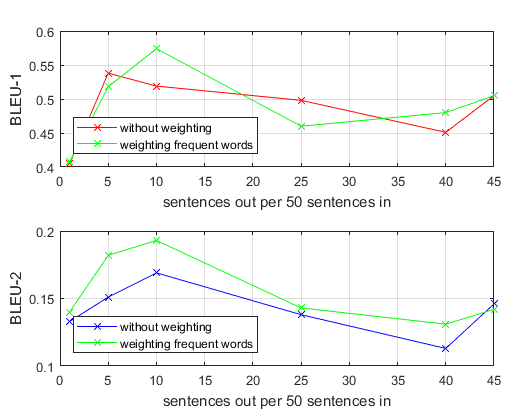
\includegraphics[width=1\linewidth]{bleus_good}
	\caption{BLEU scores for varying the compression ratio per recursive cycle for the Alchemist.}\label{fig:bleus}
\end{figure}

\begin{table}[H]
	\centering
	\caption{ROUGE results of summaries for The Alchemist}\label{tab:rouge-alchemist}
	\begin{tabular}{l l l l}
		\toprule
		\textbf{}   & \textbf{ROUGE-1} & \textbf{ROUGE-2} & \textbf{ROUGE-SU4} \\ \midrule
		CliffsNotes & 0.350           & 0.000           & 0.087 \\ \midrule
		SparkNotes  & 0.652           & 0.273           & 0.295 \\ \midrule
		GradeSaver  & 0.105           & 0.000           & 0.031 \\ \midrule
		Our summary & 0.120           & 0.042           & 0.045 \\
		\bottomrule
	\end{tabular}
\end{table}

